\chapter{Graph Theory}
Now in normal language, Graph refers to a paper with a grid of squares. In more formal language we define it as follows:\\
A graph is a mathematical object we use to think about networks. It consists of a bunch of points, called vertices, and lines joining pairs of vertices, called edges.\\
While it is not 'explicitly' required in Olympiads, it makes easy work of a lot of problems which would otherwise be a lot harder. Also it's an active area of research so familiarity with it would not hurt.\\
\section{Definitions}
As I mentioned above, graphs are usually networks. We usually let $G$ denote the graph, $V$ the set of vertices and $E$ the set of edges, and write $G = (V, E)$.
\begin{figure}[h]
    \centering
    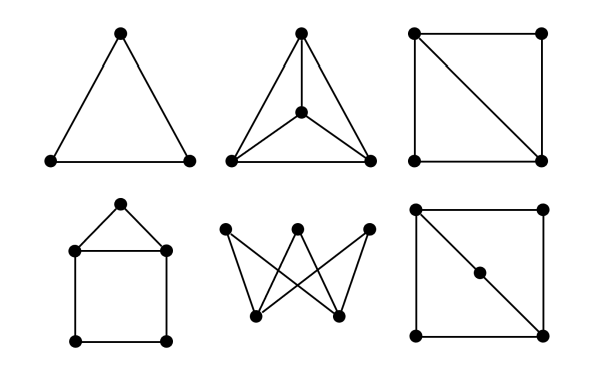
\includegraphics[width=0.5\linewidth]{Photos/Small graphs.png}
    \caption{Some graphs}
\end{figure}
We say two vertices are adjacent or are neighbors if they are joined by an edge, and nonadjacent otherwise. We say an edge and a vertex are incident if the vertex is one of the endpoints of the edge. The degree of a vertex $v$ is the number of edges incident with $v$.\\
\begin{example}
    What is least number of edges a graph on n vertices can have? What is the most number of edges a graph on n vertices can have?
\end{example}
The least number will be 0, as that will just be some points on a plane, with no edges joining them. That's called an independent set or empty graph.\\
The most will be $\binom{n}{2}$ where every node is attached to every other node. This is called a clique graph or a complete graph.\\
Believe it or not, with so little theory, we are now ready for our very first theorem. \\
\begin{theorem}
Let $G = (V, E)$ be a graph. Then:
\[ \sum _{v\in V}\deg v=2|E| \]
\end{theorem}
The proof is quite trivial. The LHS counts the degree of every vertices, which will be twice the number of edges as every vertices has 2 edges, which will both add it to the total. This is called the Handshake lemma as we can let the vertices be the number of people in a corporate boardroom and the edges be the handshake between them. If we ask every person how many hands he shook(the degree of his vertices) and add it up, it is quite elementary that we'll get twice the number of handshakes.\\
\begin{example}
     Is there a family of graphs such that every vertex has degree 0? 1? 2? 1 or 2? $\clubsuit$ Given integers $p$ and $q$, is there a graph such that every vertex either has degree $p$ or $q$
\end{example}
\begin{example}
     Let a vertex be even if it has even degree, and odd if it has odd degree. Which of the following doesn't exist: \\
     \begin{enumerate}
         \item Graph with only even vertices
         \item Graph with only odd vertices
         \item Graph with exactly one even vertex
         \item Graph with exactly one odd vertex
     \end{enumerate}
\end{example}
\section{Paths and Walks}
A walk in a graph $G$ is a sequence of vertices $v_0 - v_1 - v_2 - \dots - v_n$ such that each vertex $v_i$ is adjacent to the vertex $v_{i-1}$ before it and the vertex $v_{i+1}$ after it. We call $L$ the length of the walk.\\
A path in a graph $G$ is called a walk if all the vertices are different. Basically, every walk is a path, but every path is not a walk.\\
This leads us to ask: Given a walk between two vertices in a graph, how do we obtain a path between them? Is there always a walk between two vertices in a graph?\\
The answer is trivial, if a walk has cycles where we start a $v_n$ and after exploring some more vertices end at $v_n$, we can just remove them and have a path.\\
The answer to the second one is simple: no. For example in an independent set, we'll obviously not have a walk between any two points. \\
This leads us to a few more definitions:\\
\begin{definition}
    A cycle in a graph G is a sequence of vertices $v_0 - v_1 - v_2 - \dots  - v_n = v_0$ such that each vertex $v_i$ is adjacent to the vertex $v_{i-1}$ before it and the vertex $v_{i+1}$ after it. We call $L$ the length of the cycle.
\end{definition}
\begin{definition}
    A graph is disconnected if it can be divided into two parts with no edges between the parts, otherwise it is connected.
\end{definition}
\begin{definition}
    A connected component of a graph is a connected subgraph which is as large as possible.
\end{definition}
\begin{definition}
    Let $G$ be a connected graph. A cut vertex in $G$ is a vertex whose removal disconnects the graph. A cut edge in $G$ is an edge whose remove disconnects the graph
    \begin{figure}[h]
        \centering
        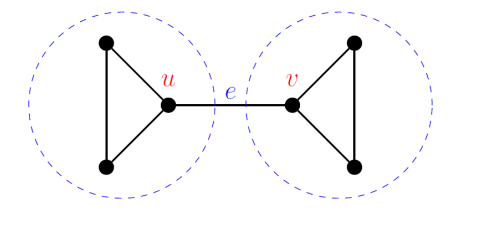
\includegraphics[width=0.5\linewidth]{Photos/Cut vertex.png}
        \caption{$e$ is the cut edge and $u,v$ the cut vertices}
        
    \end{figure}
\end{definition}
And now a theorem
\begin{theorem}
    If a graph has a cut edge, it has a cut vertex.\\
    However the converse of this is not true. If it has a cut vertex, it may or may not have a cut edge.
\end{theorem}
\begin{proof}
    The theorem is trivial for a $graph$ with less than $3$ vertices.\\
    Let $G$ have more than 3 vertices, and the cut edge $e=uv$. The other vertices will have a path to either $u$ or $v$ without using $e$ but not both as that would violate the assumption that $e$ is the cut edge.\\
    Here if one of $u$ or $v$ is removed, the graph would get disconcerted. If and only if $\deg u$ or $\deg v$ is zero, it will not be a cut vertex(which can happen for only one of them).\\
    The converse of this theorem is however not true. A counterexample will suffice:
    \begin{figure}[h]
        \centering
        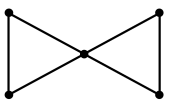
\includegraphics[width=0.5\linewidth]{Photos/counterexample.png}
        \caption{The Counter-example}
    \end{figure}
\end{proof}
\begin{example}
    Let G be a graph with $n \geq 2$ vertices such that every vertex has degree at least $\frac{n-1}{2}$. Show that G is connected.
\end{example}
\section{Trees}
\begin{example}
    What is the smallest number of edges a connected graph of $n$ vertices can have?
\end{example}
If you try to draw connected graphs with the fewest number of edges possible, you’ll start to notice that they have a particular structure. They should, if you look closely, look like trees. \\
\begin{definition}
    A graph is acyclic if it contains no cycles. We call an acyclic graph a forest, and a connected acyclic graph a tree. A leaf is a vertex in a tree with degree one.
\end{definition}
All trees are forests, but all forests are not trees.\\
\begin{figure}[h]
    \centering
    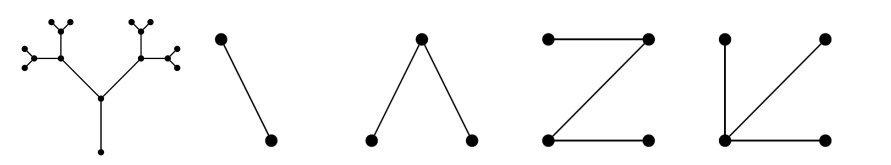
\includegraphics[width=0.5\linewidth]{Photos/trees.png}
    \caption{Some trees}    
\end{figure}
You would have noticed that the number of edges in a tree of $n$ vertices is $n-1$.  You should also notice that every edge is a cut edge. Another thing that is elementry to note is that adding any new edge will create a cyclic path. A less obvious fact, however, is:\\
\begin{theorem}
    A forest with $n$ vertices and $k$ components contains $n - k$ edges
\end{theorem}
\begin{proof}
    Forest is called forest as every component will be a tree(as in real life). So we have $k$ trees which in total have $n$ vertices. Let the individual trees have $n_1, n_2, n_3 \dots n_k$ vertices and $n_1+n_2+n_3\dots +n_k=n$, so the number of edges will be $n_1 -1 +n_2 -1 + n_3 -1 \dots n_k -1= n-k$\\
\end{proof}
Let's now talk about one very last topic, and the very reason why we studied trees.
\begin{definition}
    A spanning tree of a graph $G$ is a subgraph of $G$ that is a tree containing all the vertices of $G$.
\end{definition}
The fun fact is:\\
\begin{theorem}
    A graph is connected if and only if it has a spanning tree.
\end{theorem}
\begin{proof}
As the statement has if and only if, we'll need to prove the theorem as well as its converse. \\
Let's first prove that if $G$ has a spanning tree it is connected. Suppose $G$ has a spanning tree. Then $G$ is connected, since for every pair of vertices $u, v$ there is a path from $u$ to $v$, namely the path in the spanning tree.\\
Now we'll prove that every connected graph has a spanning tree.\\ Suppose $G$ is connected. Let $e1, e2, \dots, e_m$ be the edges of $G$ in some order. If we go through the edges of $G$ in order and remove edge $e_i$ which is in a cycle then we end up with a graph $G'$
It it trivial that $G'$ is connected (if we remove $e_i$ then since $e_i$ is in a cycle the remaining graph is still connected). If we break all such cycles, we'll be left with $T$ which will be the spanned tree of graph $G$. 
\end{proof}
\begin{example}
    How many spanning trees does a tree have? How many spanning trees does a cycle have? How many spanning trees does a complete graph have?
\end{example}
\section{Real life applications}
I had promised in the start that graph theory has a varity of real lie applications. We'll go through a few here.\\
One application of paths in graphs is finding driving directions. Let's say I want to go from Cambridge University to Mathematics Bridge.  What is the fastest way to get there?
\begin{figure}[h]
    \centering
    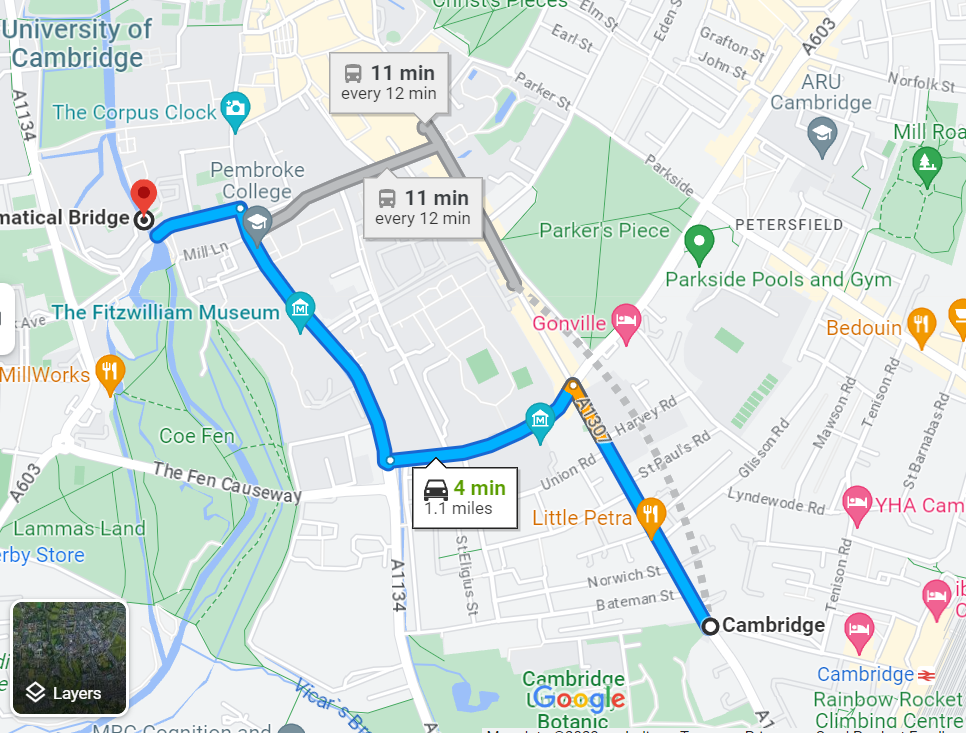
\includegraphics[width=0.5\linewidth]{Photos/map.png}
    \caption{The google map}
\end{figure}
We can formulate this problem as a graph theory problem, where $G = (V, E)$ is a graph whose vertices $V$ are intersection points between roads in Cambridge, and edges are road segments. Then we can think of the university and Math Bridge as two vertices $u$ and $v$ in my graph $G$, and my questions become the following: How can we find whether there is a path between $u$ and $v$? How can we find a shortest path from $u$ to $v$?\\
We can do this in many ways, the most basic being the depth-first search and the breadth-first search algorithm.\\
\subsection{Depth-first search}
The idea of depth first search is: : Start at $u$ and ‘keep walking’, i.e. walk as far as possible searching for $v$, and if you hit a dead end backtrack.\\
The algorithm is as follows: Start at$u$ and move to any of it's neighbours. Let this be $v'$. Now from $v'$ move to another neighbour other than $u$. The algorithm stops on three conditions:\\
\begin{enumerate}
    \item If it reaches $v$, it then returns the path as the output.
    \item If it reaches a $v'$ with no unvisited neighbours. It will retract its path and move till the next fork where it will make a new choice and try again.
    \item If it reaches $v'=u$ and has no unvisted neighbours, it will declare that we have no path from $u$ to $v$
\end{enumerate}
Depth-first search allows us to find a path from u to v, or verify that no such path exists. But the path it finds has no guarantee of being the shortest path. In sad cases, it may generate a path from Cambridge to Kings Collage and then to the bridge.\\
\subsection{Breadth-first search}
The idea od Breadth first search is: Start at $u$, keep track of the vertices ‘closest’ to $u$ ($u$’s neighbors) and see if they’re $v$. If not, see if any of vertices ‘second-closest’ to $u$ (neighbors of $u$’s neighbors) are $v$. Eventually we'll find $v$.\\
This method is superior to depth search in the aspect that it will find the path with least number of edges. However, it also assumes that there is a path from $u$ to $v$, which if untrue, it will not detect and go till the system crashes(or it reaches a point where all vertices are neighbour less and terminates and declares no path).\\
However, they both don't give us the fastest path as we are taking all edges as equal. But roads are of different lengths and we know that longer roads take more time to travel. According to both of or methods, we'll end up considering Saudi's Highway 10(256 km) as just as short as Scotland's Ebenezer Place(2.46 meters).\\
To capture this, I will need the concept of weighted edges. A weighted graph is a graph where each edge is assigned a number, $w$ called its weight. For an edge $e$ we let $\omega(e)$ denote its weight.
\subsection{Dijkstra’s Algorithm}
The idea of Dijkstra is Start at $u$, for each vertex $v'$ keep track of an estimated (weighted) distance from $u$ to $v$. Visit the vertices in order of how ‘close’ they are to$u$ and see if they’re $v$. The more nitty gritty of this is left to the diligent reader.\\
However, despite being quite efficient, google maps doesn't work on Dijkstra. It instead uses $A^{*}$ algorithm. It basically makes the estimation step more accurate. Google also uses bi-directional search to make it quicker(looking for path from $u$ to $v$ as well as $v$ to $u$ simultaneously hoping that they meet somewhere in the middle) along with a lot of trade secret pruning, shortcuts and caching. But that is more computer science and less math.\\

\begin{xcb}{Exercises}
\begin{enumerate}
        \item Prove that for any graph with $n$ vertices and $m$ edges, has the lowest $\deg v \leq \frac{2m}{n}$ and the highest $\deg v \geq \frac{2m}{n}$.
        \item . Is it possible to build a house with exactly eight rooms, each with three doors, and such that exactly three of the house’s doors lead outside?
        \item The complement of a graph $G$ is the graph $G$ obtained by including an edge if and only if it was not present in the original graph. Prove that between $G$ and $G'$, one and only one is connected.
        \item Show that at any party, there are always at least two people with exactly the same number of friends at the party.
        \item(Martin Gardner) My wife and I recently attended a party at which there were four other married couples. Various handshakes took place. No one shook hands with oneself, nor with one's spouse, and no one shook hands with the same person more than once. After all the handshakes were over, I asked each person, including my wife, how many hands he (or she) had shaken. To my surprise each gave a different answer. How many hands did my wife shake?
        \item(IMOSL 2001) Define a $k$-clique to be a set of $k$ people such that every pair of them are acquainted with each other. At a certain party, every pair of 3-cliques has at least one person in common, and there are no 5-cliques. Prove that there are two or fewer people at the party whose departure leaves no 3-clique remaining
        \item (Italy 2007) Let $n$ be a positive odd integer. There are $n$ computers and exactly one cable joining each pair of computers. You are to color the computers and cables such that no two computers have the same color, no two cables joined to a common computer have the same color, and no computer is assigned the same color as any cable joined to it. Prove that this can be done using $n$ colors.
        \item {USAMO 2007, edited} An animal with n cells is a connected figure consisting of $n$ equal-sized cells which are square(a $n-$tile polymino). A dinosaur is an animal with at least 2023 cells. It is said to be primitive if its cells cannot be partitioned into two or more dinosaurs. Find the maximum number of cells in a primitive dinosaur
        \item Show that the Petersen graph has 2000 spanning trees 
\begin{figure}[h]
        \centering
        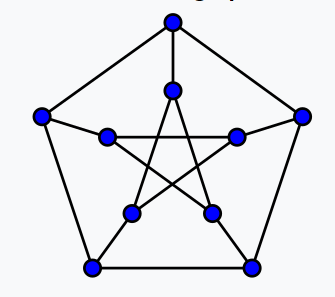
\includegraphics[width=0.5\linewidth]{Photos/Petersen Graph.png}
        \caption{Petersen Graph}
    \end{figure}
    \item (Cayley's Formula) A labelled tree of $n$ vertices is a tree of $n$ vertices where all vertices are given distinct labels from $1$ to $n$. Prove that there are $n^{n-2}$ labelled trees of $n$ vertices.
    \item(Veblen's Theorem) Prove that the edges of a graph can be partitioned into cycles if and only if each vertex has even degree.
    \item(Euler's Formula) Prove that given graph $G$ be a connected planar graph with $V$ vertices, $E$ edges and $F$ faces(number of parts it divdes the plane into, note: the outside of graph is also a face). Then $F + V - E = 2$
    \item (IrMO 1989) . Each of the $n$ members of a club is given a different item of information. They are allowed to share the information, but, for security reasons, only in the following way: A pair may communicate by telephone. During a telephone call only one member may speak. The member who speaks may tell the other member all the information he or she knows. Determine the minimal number of phone calls that are required to convey all the information to each other.
    \item (IrMO 1994) If a square is partitioned into n convex polygons, determine the maximum number of edges present in the resulting figure.
    \item (IMO 2019, edited) A social network has 2023 users, some pairs of which are friends (friendship is symmetric). If $A, B, C$ are three users such that $AB$ are friends and $AC$ are friends but $BC$ is not, then the administrator may perform the following operation: change the friendships such that $BC$ are friends, but $AB$ and $AC$ are no longer friends. Initially, $1011$ users have $1012$ friends and $1012$ users have $1011$ friends. Prove that the administrator can make a sequence of operations such that all users have at most 1 friend.
    \item (Moser's Circle Problem) Given $n$ points on the circumference of pizza, what is the maximum number of parts the circle is separated  by the chords connecting all the $n$ points to each other? (Note: \cancel{Don't} use Engineer's induction)
    \end{enumerate}
\end{xcb}